\documentclass[12pt]{article}
\usepackage{natbib}
\usepackage{url}
\usepackage[utf8x]{inputenc}
\usepackage{graphicx}
\graphicspath{{images/}}
\usepackage{parskip}
\usepackage{fancyhdr}
\usepackage{vmargin}
\setmarginsrb{3 cm}{2.5 cm}{3 cm}{2.5 cm}{1 cm}{1.5 cm}{1 cm}{1.5 cm}

\title{Visualizing 10 Years (2005-2015) of Life in Hampton Roads}								% Title
\author{Prasanna Sajjan}								% Author
\date{\today}											% Date

\makeatletter
\let\thetitle\@title
\let\theauthor\@author
\let\thedate\@date
\makeatother

\pagestyle{fancy}
\fancyhf{}
\rhead{\theauthor}
\lhead{\thetitle}
\cfoot{\thepage}

\begin{document}

%%%%%%%%%%%%%%%%%%%%%%%%%%%%%%%%%%%%%%%%%%%%%%%%%%%%%%%%%%%%%%%%%%%%%%%%%%%%%%%%%%%%%%%%%

\begin{titlepage}
	\centering
    \vspace*{0.5 cm}
    
\includegraphics[scale = 0.75]{ODU.png}\\[1.0 cm]	% University Logo
    \textsc{\LARGE Department of Computer Science}\\[2.0 cm]	% University Name
	\textsc{\Large Master's Project}\\[0.5 cm]				% Course Name
	\rule{\linewidth}{0.2 mm} \\[0.4 cm]
	{ \huge \bfseries \thetitle}\\
	\rule{\linewidth}{0.2 mm} \\[1.5 cm]
	
	\begin{minipage}{0.4\textwidth}
		\begin{flushleft} \large
			\emph{Author:}\\
			\theauthor
			\end{flushleft}
			\end{minipage}~
			\begin{minipage}{0.4\textwidth}
			\begin{flushright} \large
			\emph{Advisor:} \\
			Dr. Michele C. Weigle									% Your Advisor Name
		\end{flushright}
	\end{minipage}\\[3 cm]
	
	{\large \thedate}\\[2 cm]
 
	\vfill
	
\end{titlepage}

\chapter{\Large\selectfont\textbf{Acknowledgments}} \\\\

I take this opportunity to express my immense gratitude towards my project advisor \textbf{Dr. Michele C. Weigle}, Associate Professor, Department of Computer Science, Old Dominion University, without whom this project would have been arduous task. Her step-by-step guidance, useful suggestions and creative ideas made it much easier for me to keep track of my progress and helped me to eventually finish this project. She has been extremely understanding and supportive. \\

I want to thank \textbf{Mr. James Clary} from the Hampton Roads District Planning Commission for originally proposing this idea and providing all the data sources required for this project. I would like to acknowledge the work done by \textbf{Shawn and Valentina Jones} in creating the map of Hampton Roads using D3.js, whose work I have used in my project. \\

Finally, I would like to thank the \textbf{Department of Computer Science} for providing all the resources to complete this project.

\pagebreak

%%%%%%%%%%%%%%%%%%%%%%%%%%%%%%%%%%%%%%%%%%%%%%%%%%%%%%%%%%%%%%%%%%%%%%%%%%%%%%%%%%%%%%%%%

\tableofcontents
\pagebreak

%%%%%%%%%%%%%%%%%%%%%%%%%%%%%%%%%%%%%%%%%%%%%%%%%%%%%%%%%%%%%%%%%%%%%%%%%%%%%%%%%%%%%%%%%

\section{Preface}
The goal of this project is to analyze different data sources from U.S. Bureau of Labor Statistics, U.S Census Bureau and Virginia Department of Education, gather insights about the data and make these data insights actionable through high-quality visualizations. 

This project also aims to fulfill the goals addressed by the Hampton Roads Planning District Commission (hereby referred to as HRPDC), who provided the links to all the data sources.  Below are the list of goals that were laid out by HRPDC:

\begin{itemize}

\item Indicate visually the change in	and	size of	employment by industry over time with the relative incomes of those	industries
\item Measuring	the	change in incomes of the industry along	with changes in	employment 
\item Indicate visually	the	change	in	employment	by	occupation	over time along	with the relative incomes of the occupation
\item Examine the changes in graduation	rates for each of the localities in Hampton Roads
\item Show the flows of commuters throughout the region of Hampton Roads

\end{itemize}

\newpage

\section{Motivation}
The idea was originally proposed by  Mr. James Clary, Senior Economist at HRPDC in Dr. Weigle's Spring 2015 class, Information Visualization. Mr. Clary does not hold the position of Senior Economist at HRPDC anymore. Folks at HRPDC wanted to see trends in income and employment data spread across different industries and occupations, over time. They also wanted to know about the different high school graduation rates and commuting patterns in the Hampton Roads area.

They wanted to use the results from this project and then compare it with the overall average of U.S, to see where things need to be improved. I was also curious myself to know about the area I have lived in for the past 2 years and also my passion about dealing with large data sets and converting them into meaningful visualizations led me to do this project.

\newpage

\section{Data Sources}
For the data on income and employment for different industries and occupations, I referred to the ``Bureau of Labor Statistics''. Links to the same can be found below: 
\begin{itemize}
\item Quarterly Census of Employment and Wages - \url{(http://www.bls.gov/cew/datatoc.htm)}  
\item Occupational Employment Statistics - \url{(http://www.bls.gov/oes/current/oes_47260.htm)}
\end{itemize}
\begin{figure}[htp]
\centering
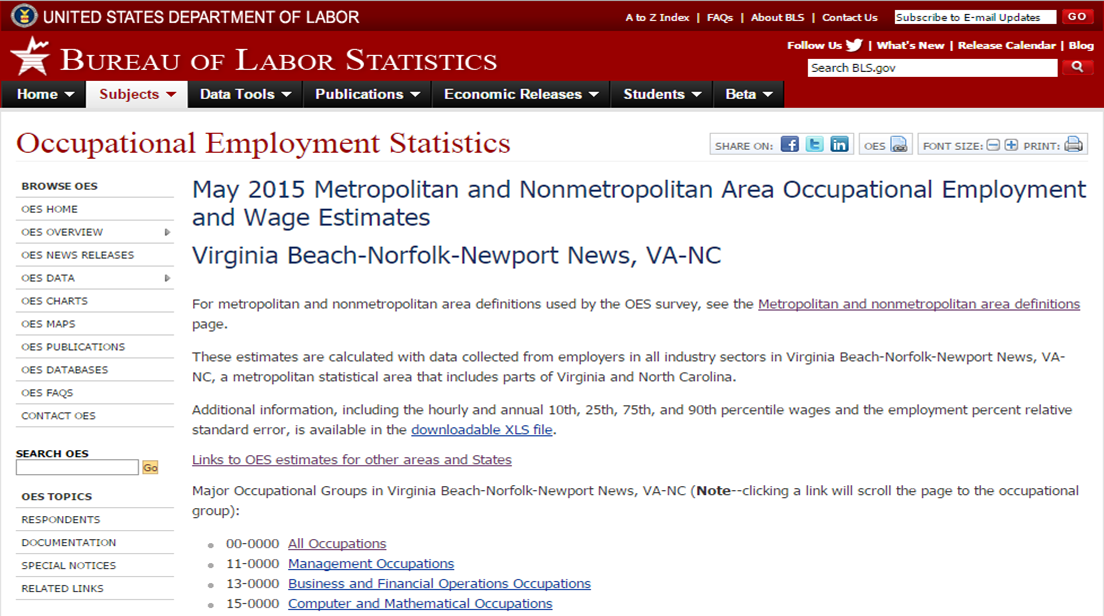
\includegraphics[scale = 0.35]{OCC.png}
\caption{Snapshot of Occupational Data}
\label{highq}
\end{figure}
\begin{figure}[htp]
\centering
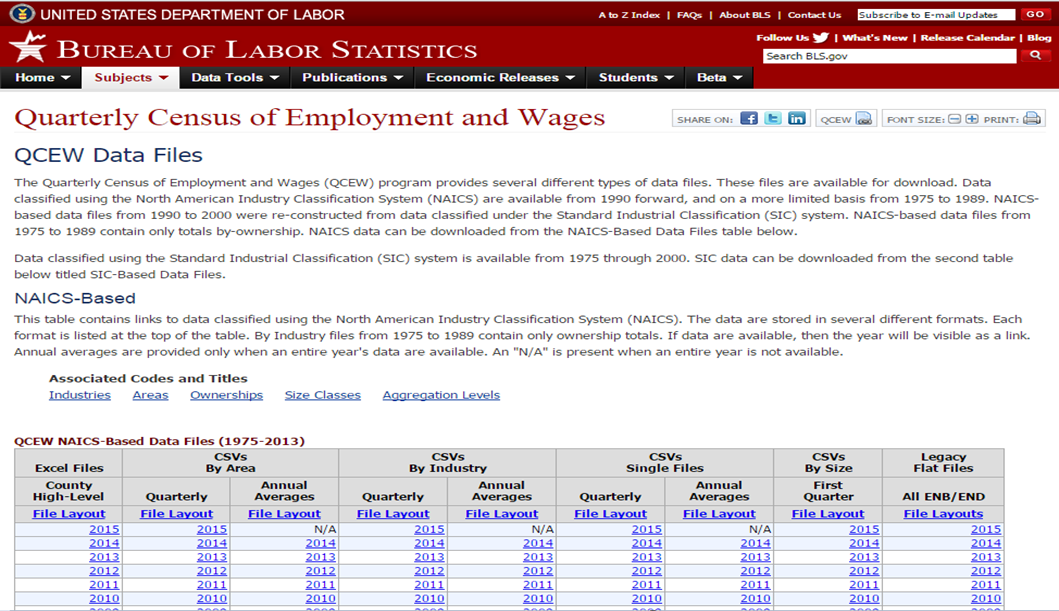
\includegraphics[scale = 0.35]{IND.png}
\caption{Snapshot of Industry Data}
\label{highq}
\end{figure}
\newpage

For the data on commuting patterns and high school graduation rates, I referred to U.S Census Bureau and Virginia Department of Education.Links to the same can be found below: 
\begin{itemize}
\item American Community Survey and Decennial Census Journey to work data  - \url{(https://www.census.gov/hhes/commuting/data/commutingflows.html)}  
\item Virginia Cohort Reports - \url{(http://www.doe.virginia.gov/statistics_reports/index.shtml)} \\\\
\end{itemize}
\begin{figure}[htp]
\centering
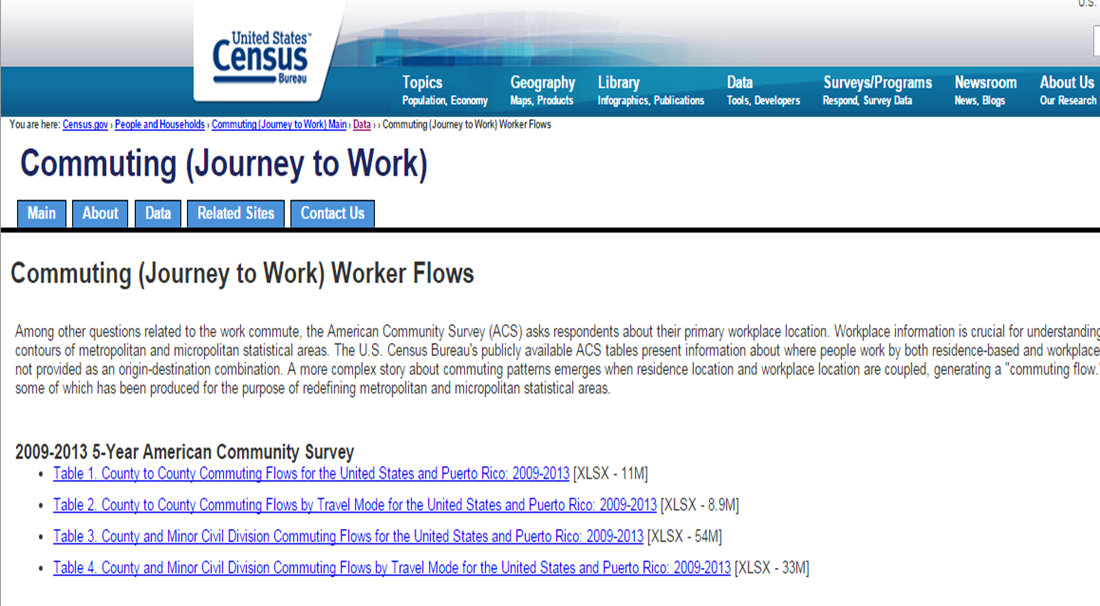
\includegraphics[scale = 0.35]{COMM.png}
\caption{Snapshot of Commuting Data}
\label{highq}
\end{figure}
\begin{figure}[htp]
\centering

\includegraphics[scale = 0.35]{GRAD.png}
\caption{Snapshot of Graduation Data}
\label{highq}
\end{figure}
\newpage

\section{Data Set and Cleaning}
Data-sets were available in the form of Excel spreadsheets from all the data sources. Some of the spreadsheets were direct downloads whereas others were available part of a zip package. There were roughly 50,000 - 160,000 records on each of the spreadsheet. All the data was structured and each column carried a heading using standard naming conventions according to the respective Bureau.

Even though the data was structured, the format was not consistent throughout all the years. This made it hard for me to automate the process of cleaning the data. There are plenty of libraries available in Python\footnote[1]{http://www.python-excel.org/} to manipulate excel files, but due to the inconsistency in the format of the data, I chose to clean the data manually. It did take me more time to do it this way, but in the end I was able to clean the data the way I wanted. I got rid of the standard headers and used my own naming for easier understanding. I used data filters in Excel to get what I want. Below is an example of the data inconsistency - \\

\begin{figure}[htp]
\centering
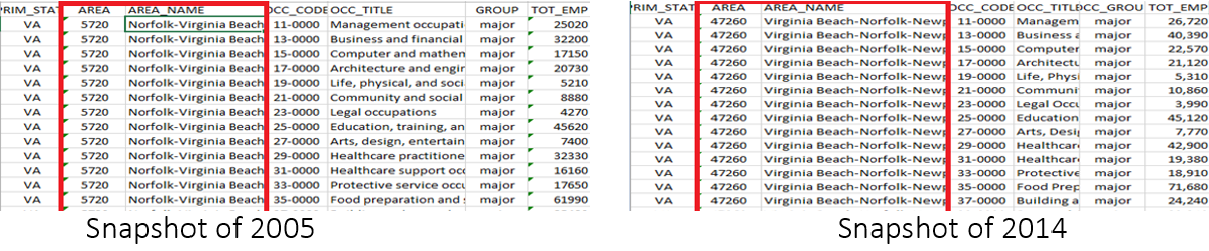
\includegraphics[scale = 0.5]{DATA.png}
\caption{Example of Data inconsistency}
\label{highq}
\end{figure}

\newpage

\section{Overview of the System}

The whole system was split into 4 different sub-systems. I used a combination of Tableau\footnote[2]{http://www.tableau.com/} and D3.js\footnote[3]{https://d3js.org/} to create all the visualizations. To see the trends in ``Income and Employment by Industry'' I created line charts to show the change in and size of income and employment over time and barc harts to measure these changes on a percentage scale. To see the trends in ``Income and Employment by Occupation'', I created line charts to show the change in and size of income and employment over time. All of this was achieved using Tableau and Microsoft Excel. 

In order to show the trends in high school graduation rates, I created interactive line charts to exam the changes by each locality. I also used a combination of Choropleth map\footnote[4]{A choropleth map is a thematic map in which areas are shaded or patterned in proportion to the measurement of the statistical variable being displayed on the map, such as population density or per-capita income - \url{https://en.wikipedia.org/wiki/Choropleth_map}} and static line charts to display the graduation rates for each locality based on factors such as gender, race and socio-economic factors. Users can click on the region they are interested in on the map and it will show the line charts accordingly. 

\begin{figure}[htp]
\centering
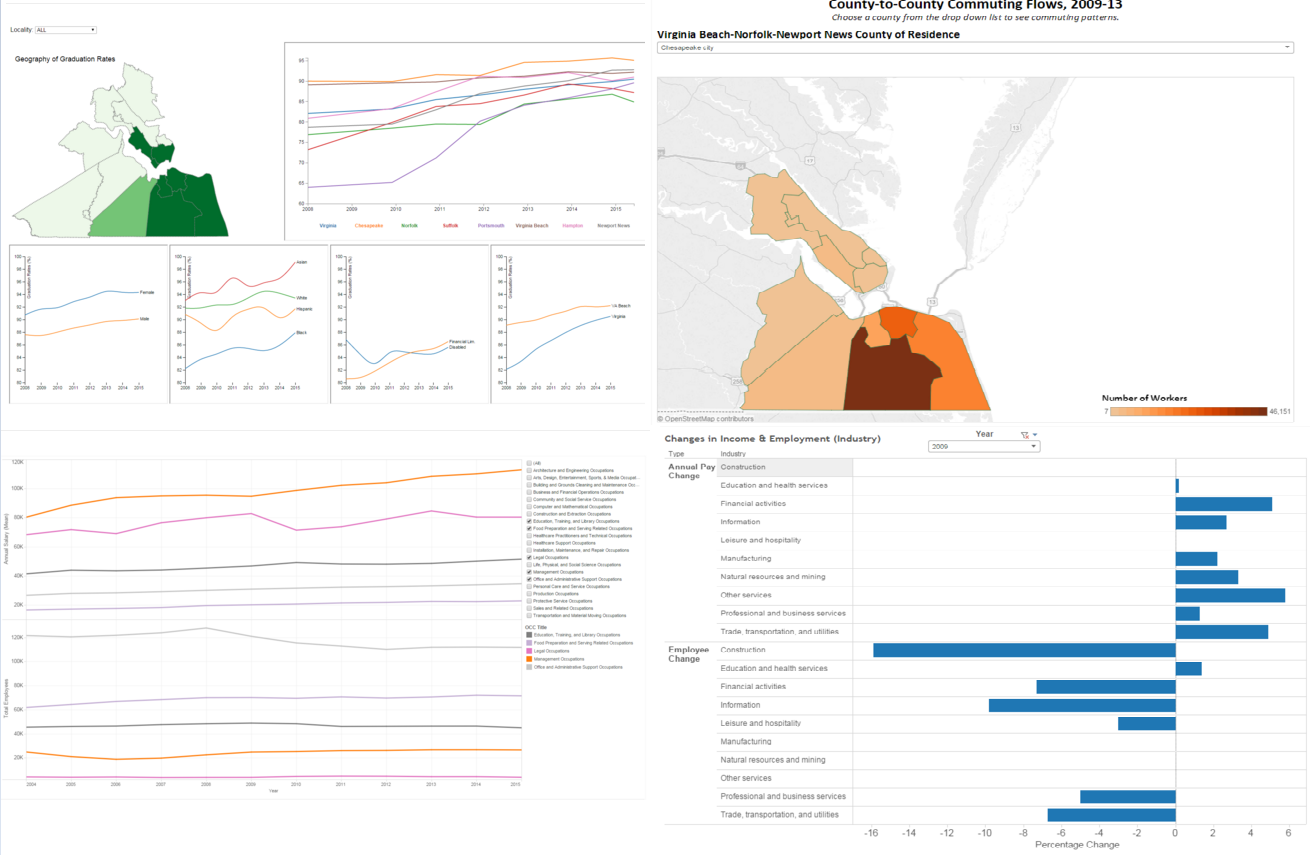
\includegraphics[scale = 0.35]{Overall.PNG}
\caption{Overview of the System}
\label{highq}
\end{figure}

\newpage

To achieve this I used D3.js, JSON, HTML, CSS, jQuery and JavaScript. In order to show the commuting patterns in Hampton Roads, I created a Choropleth map using Tableau and included tooltip to highlight the number of commuters in each region. I had to find out the latitude and longitude of each cities and then use that to draw the map in Tableau. To find out the latitudes and longitudes, I used this website - \url{http://www.latlong.net/}

Finally, all the sub-systems were put together into one main system using Bootstrap\footnote[5]{http://getbootstrap.com/} framework. I have listed down all the goals for each system and the valuable insights that I gained from each system besides it. All of this can be viewed on the project website which can be accessed by following this link - \url{www.cs.odu.edu/~psajjan/cs698/}

\newpage

\section{Insights}
After developing all the visualizations, I started examining each of them individually to see if I could gain some meaningful insights from it. I carefully observed each of the sub-systems and have listed down all my insights regarding each of the sub-system below - 

\subsection{Income and Employment by Industry}
\begin{itemize}

\item \textbf{Trade, transportation and utilities} industry employed the highest number of people whereas \textbf{Natural resources and mining} industry employed the least number of people. 
\item \textbf{Manufacturing} industry had the highest annual pay whereas \textbf{Leisure and hospitality} industry had the lowest annual pay.
\item After the ``Great recession''\footnote[6]{\url{https://en.wikipedia.org/wiki/Great_Recession_in_the_United_States}} in the U.S, all the industries experienced a decline in the number of employment but Education and health services saw a steady increase
\item \textbf{Construction} industry had the highest impact from the ``Great recession'', where there was a 16\% decline in employment in the year 2009.
\end{itemize}

\subsection{Income and Employment by Occupation}
\begin{itemize}

\item \textbf{Office and administrative} support occupation had the highest number of employees whereas \textbf{Legal} occupation had the least number of employees. 
\item \textbf{Management} occupation paid the highest annual salary whereas \textbf{Food preparation and serving} related occupation paid the lowest annual salary.
\item The ``Great recession'' did not have a major impact on any of the occupations since the trends looked steady over the period of 10 years.

\end{itemize}

\newpage

\subsection{High school Graduation rates}
\begin{itemize}

\item \textbf{Chesapeake} city had the highest graduation rates and way above Virginia state's average graduation rate, whereas \textbf{Portsmouth} city had the lowest graduation rates. 
\item \textbf{Females} dominated over males in each of the 7 counties, \textbf{White} and \textbf{Asian(minority)} race had the highest graduation rate among all the races.

\end{itemize}

\subsection{Commuting Patterns}
\begin{itemize}

\item \textbf{Virginia Beach} city had the highest number of daily commuters(226,779), whereas Mathews county had the lowest
number of daily commuters(3,422)
\item \textbf{Norfolk} city had the highest retention rate, where 67.63\% of the city's daily commuters worked within the city and York county had the lowest, where 27.89\% of the commuters worked within the county.

\end{itemize}

\newpage

\section{WHAT-WHY-HOW Framework}

\begin{figure}[htp]
\centering
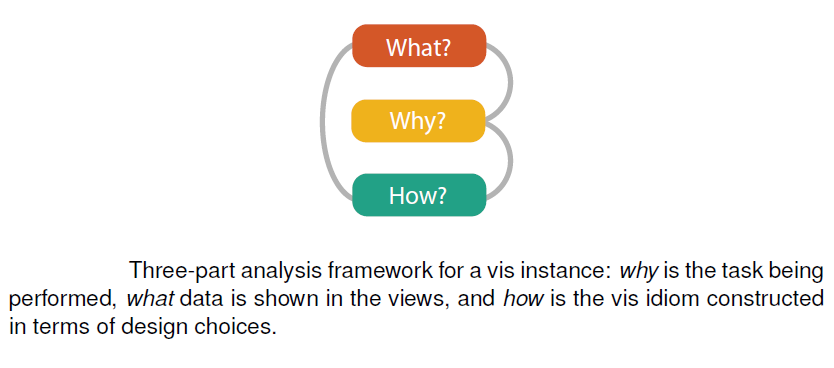
\includegraphics[scale = 0.5]{WWH.PNG}
\caption{Overview of What-Why-How Framework}
\label{highq}
\end{figure}

The What-Why-How framework described by Tamara Munzner in her ``Visualization Analysis and Design'' textbook, acts as a basic guideline and framework for visualization any form of data. I will discuss how this framework was effectively applied in
my project below - 

\subsection{What: Data}

All the data-sets were tables with multiple attributes and items. All these tables were stored in Excel spreadsheets. The entire data-set was a static file. Here, the attributes will be used as filters and items are the values for each attribute. The attribute types are categorical attributes and quantitative attributes. The Choropleth map developed using Tableau uses the latitude and longitude to represent each county/city in the area. For the map created using D3.js, I borrowed code from Shawn and Valentina Jones'\footnote[7]{https://github.com/shawnmjones/hr-contracting} Github repository and modified it according to my needs. The bar-charts and line-charts use quantitative data.

\subsection{Why: Actions and Abstract Tasks}

Based on the list of actions available my visualization uses analyze and query actions. The users can analyze the data and discover some interesting patterns. The user can also query the visualization by using the different filters available and summarize them. The viewers can perform cross-attribute comparison, for example comparing different industries and occupations.

\subsection{How: Encode}
 
Most of the colors used in my visualizations are color blind safe. In the Choropleth map, the channel hue is used to show the count of commuters for each city/county. The channel area is used to encode the quantitative income and salary data in the form of line charts and bar charts. Different color coding is used for each industry and occupation in the line charts.

\subsection{How: Reduce/Manipulate}

In order to perform reduction the users can perform dynamic filtering and aggregation using the filters provided. Viewers can
also zoom in and out to view the name of the states or countries on the Chorpleth map.

\newpage

\section{Challenges}
Overall, I had a lot of fun working in this project but there were a few challenges which made some of the tasks difficult to achieve. These were minor challenges and nothing major to deviate entirely from the project's idea. Below are the list of some of the minor challenges that I came across while I was working on the project - 

\begin{itemize}

\item Data inside the Excel spreadsheets was structured but not easy to read. What I mean by this is, even though the data was structured into rows and columns, the column headers for each of the columns were not easy to read. They were named using standard conventions followed by each of the government agency and the expansion of these headers was not available inside the spreadsheet. I had to manually go look for them on the website, which was located at an entirely different location.

\item Initially I thought I could just use the name of the cities and counties to draw the map through Tableau. But, later I found out it was only possible by finding out latitudes and longitudes of each city/county in order to draw the map using Tableau. Then I used latlong.net to find the latitude, longitude of each city and county.

\item Even though Mr. Clary shared a document with all the links to the data sources, they were not direct links. It is very easy to get lost of a government website and figure out where you are. I had to browse through different sections of the websites to finally arrive at the place and find the data-sets I was looking for. 

\end{itemize}

\newpage

\section{Future Work}

Even though the work done in this project is substantial, it can be further improved upon as explained below - 

\begin{itemize}

\item The data sources that are mentioned above are available for all the regions in the U.S and not just Hampton Roads. Hence, the study made in this project can be expanded to any region in the U.S

\item We only studied the graduation patterns in the Hampton Roads area and showed the trends visually. Further work can be done to study the factors affecting these graduation rates such as cost of living, crime rate in the area, total household income etc.

\item With respect to commuting patterns, data shows that some people living in Hampton Roads actually commuted to other states out of Virginia. This can be shown on the map since in my current project, I only show commuting patterns within the Hampton Roads area.

\end{itemize}

\bibliographystyle{plain}
\bibliography{biblist}

\end{document}